%\documentclass[10pt]{report}

%\usepackage[margin=2.5cm]{geometry}
%\usepackage{tikz}
%\usetikzlibrary{shapes,arrows}
%\usepackage{amsmath}
%\usepackage{array}
%\usepackage{subfigure}
%\usepackage[colorlinks=true,linkcolor=blue]{hyperref}
%%\usepackage[all]{hypcap}
%\usepackage{lscape}
%\usepackage{multirow}
%\usepackage[utf8]{inputenc}
%\usepackage[T1]{fontenc}
%\usepackage{algorithmic}
%\usepackage{algorithm}
%\usepackage{rotating}
%\setlength{\parindent}{0in}
%
%\title{Feature based classifier for Astronomical time series}
%
%\date{}
%
%\begin{document}
	%\maketitle
	
	\chapter{Supervised classification with statistical features, linear segmentation and wavelet transforms} % TODO new title
	\section{Aim}
		Supervised classifiers are an powerful and easily extensible way to incorporate many features of a data object into a classification scheme. In the context of light curve classification a variety of numerical features may be useful for discriminating between classes, from statistical properties of the flux values observed to coefficients extracted from wavelet transforms. The aim of these experiments is to assess the transient classification performance of numerical features within the experimental framework outlined in chapter~\ref{chap:experimentalframework}. As outlined in the framework chapter, each experiment will involve 10-fold cross validation with training features extracted from standardised light curves and tested on the remaining light curves with the distortions applied. The Random Forest is used as a classifier because of its robustness to confused and even contradictory features (as will occur frequently when the data is distorted) and good performance relative to other options. Performance will be evaluated in terms of F-Score, Precision and Recall microaveraged across each class. Running times for the classification post feature extraction will also be included. The results will form a baseline of classification performance to which more sophisticated features and techniques will be compared. % TODO what other classifiers did random forest beat

	\section{Method}
	This experiment follows the experimental framework outlined in chapter~\ref{chap:experimentalframework}. 10-fold cross validation is used on the set of light curves, the training light curves being undistorted and complete, and the test light curves with distortions applied as per the framework. For the implementation details see the relevant chapter.


		The supervised classification method used is the Random Forest. The Random Forest classifier is a variant of the decision tree classifier that allows the discriminative powers of the features to be exploited more fully. Instead of a single decision tree producing a class output based on a set of rules, a series of decision trees (called a \emph{Forest}) working on a few randomly chosen features each provides a vote for the class of the subject. If a pair of features have contradictory classifications for a certain class but are good at discriminating amongst others, the Random Forest will allow them to be useful at once. In preliminary experiments the Random Forest performed as well as or better than other supervised classifiers.\\ % TODO add a reference for decision tree, random forest and experiments, and this explanation (maybe a diagram), other classifiers it did better than.

	As per the evaluation section in chapter~\ref{chap:experimentalframework} experimental results will be presented as confusion matrices, tables of precision, recall and F-score, and plots of F-score versus the distortion parameter within each experiment.
	
	Additionally, each result table and plot will include subtractive analysis of the features with the removal of certain logical subsets. This will enable an effective comparison of the features used in terms of both overall and inter-class discrimination.
	
	\section{Features}
	\label{sec:baselinefeatures}
	The features used in the experiment are outlined in table \ref{tab:features} and organised into logical subsets. Features span from basic statistical metrics from histograms of flux values and linear segmentations of the light curve, to more sophisticated approaches such as wavelet transforms and periodograms, and statistical features extracted from a linear segmentation of the light curve. Justifications, visualizations and detailed descriptions of computation for the features are given in the following section.
	
	\begin{table}[ht!]
	\centering
		\label{tab:features}
	
		\begin{tabular}{|l|p{0.25\textwidth}|p{0.4\textwidth}|} \hline
		\textbf{Feature set} & \textbf{Short name} & \textbf{Description}\\ \hline
		\multirow{8}{*}{Flux statistical features}
		& \verb#flux_median# & Median deviation of flux distribution \\ \cline{2-3}
		& \verb#flux_skew# & Skew of flux distribution \\ \cline{2-3}
		& \verb#flux_kurtosis# & Kurtosis of flux distribution \\ \cline{2-3}
		& \verb#flux_min# & Minimum of flux distrubtion \\ \cline{2-3} % TODO remove comments about mean, stddev
		& \verb#flux_max# & Maximum of flux distribution \\ \cline{2-3}
		& \verb#flux_hist_pos(inc)#  for $inc$ 0.05, 0.1, 0.2, 0.3, 0.4, 0.5, 0.6, 0.75, 1, 1.5, 2, 3 & Fraction of \emph{positive} $z$-normalised flux values within $inc$ of the mean  \\ \cline{2-3}
		& \verb#flux_hist_neg(inc)# for $inc$ 0.05, 0.1, 0.2, 0.3, 0.4, 0.5, 0.6, 0.75, 1, 1.5, 2, 3 & Fraction of \emph{negative} $z$-normalised flux values within $inc$ of the mean  \\
		\hline
	\multirow{8}{*}{Segmentation statistical features}
		& \verb#grad_median# & Median of gradient distribution \\ \cline{2-3}
		& \verb#grad_skew# & Skew of gradient distribution \\ \cline{2-3}
		& \verb#grad_kurtosis# & Kurtosis of flux distribution \\ \cline{2-3}
		& \verb#grad_min# & Minimum of gradient distribution \\ \cline{2-3} % TODO remove comments about mean, stddev
		& \verb#grad_max# & Maximum of gradient distribution \\ \cline{2-3}
		& \verb#grad_hist_pos(inc)#  for $inc$ in 0.05, 0.1, 0.2, 0.3, 0.4, 0.5, 0.6, 0.75, 1, 1.5, 2, 3 & Fraction of \emph{positive} gradient values within $inc$ of the mean  \\ \cline{2-3}
		& \verb#grad_hist_neg(inc)# for $inc$ in 0.05, 0.1, 0.2, 0.3, 0.4, 0.5, 0.6, 0.75, 1, 1.5, 2, 3 & Fraction of \emph{negative} gradient values within $inc$ of the mean  \\
		\hline
		\multirow{1}{*}{Haar wavelet transform} & \verb#haar_coeffs(n)# for $n = 1 \ldots 15$ & Haar wavelet transform computed on centered light curve \\
		\hline
		\multirow{1}{*}{Lomb scargle periodogram} & \verb#lomb_phase(n)# for $n = 1 \ldots 4$ & Highest 4 Lomb-Scargle periodogram phase peaks \\ \hline
		\end{tabular}
		\caption{Basic feature set}
	\end{table}	

%	This should be in the simulated data section
%	With the use of simulated data care must be taken to prevent generic properties of a simulated class from leaking into the classifier. For example, if a particular class, say that of the Extreme Scattering Event (ESE) were a transient event occuring within a 200-day period, with all the other classes having time scales of 400, several features would allow to classifier to spot this arbitrary and unrealistic choice of time scales and would classify the ESE class much more accurately than it should. 
	

	
	% TODO justify the Random Forest
	% TODO astronomically motivated features vs. basic statistical features, time series analysis techniques
	% TODO features from "qualitative space fragmentation"

	\subsection{Flux statistical features}
	The absolute simplest features that could be useful in discriminating between astronomical light curves are statistical properties of the distribution of the magnitude or \emph{flux} of its elements. Simple statistical features were used effectively to classify periodic astronomical light curve data in \citet{richards2011machine}. Information about the variability and dynamics of a transient is encoded in the shape of a histogram produced from the flux values. As with all feature extraction approaches in this thesis the light curves will undergo a $z$-normalisation beforehand to eliminate the effects of amplitude scaling in the signal. The statistical properties we are interested in are the \emph{median}, \emph{kurtosis}, \emph{skew}, \emph{minimum} and \emph{maximum}, and the fractions of positive and negative elements of the flux set falling within predefined fractions of the standard deviation. These simple statistical features are fast to extract, very expressive, and should be somewhat robust to noise and missing data. The shape of the histogram will be affected far less under a noise distortion than features working on a point-by-point basis, such as distance measures. % (TODO ref z-normalisation) 
	
	\subsubsection{Skew and Kurtosis}
	\emph{Skew} and \emph{Kurtosis} are two statistical measures of the shape of a data distribution. Skew measures the degree of evenness in the distribution either side of the mean and for a set of flux values $f$ with mean $\bar{f}$ the skew is computed as:
	\begin{equation}
		\frac{\frac{1}{n}\sum\limits^{n}_{i=1}(f_{i} - \bar{f})^{3}}
		{(\frac{1}{n}\sum\limits^{n}_{i=1}(f_{i} - \bar{f})^{2})^{\frac{3}{2}}}
	\end{equation}
	
	Kurtosis measures the `peakiness' of the flux distribution - how strongly flux points are centered around the mean. For a flux sample $f$ with mean $\bar{f}$ the kurtosis is:
	\begin{equation}
		\frac{\frac{1}{n}\sum\limits^{n}_{i=1}(f_{i} - \bar{f})^{4}}
		{(\frac{1}{n}\sum\limits^{n}_{i=1}(f_{i} - \bar{f})^{2})^{2}} \\
	\end{equation}
	
	Figure~\ref{fig:samplestats} shows two sample light curves, their flux histograms and the corresponding skew and kurtosis.  It illustrates the discriminatory power of these simple features. \\
	
	Skew is highest (in magnitude) for sources with sudden pesaks and troughs emerging from background noise in one direction. As a result, the Supernovae light curve has a very positive skew. The Extreme Scattering Event has a slightly negative skew because of the relative intensity of the central dip to the peaks either side. For sources that are slowly varying or consistent, and skew will be closest to zero. \\
	
	Kurtosis will be highest for signals that are extremely consistent or have very sudden variations. Signals that oscillate a great deal with have much lower kurtosis. Again, the supernovae, characterised by sudden sharp increases in flux, has a very high kurtosis. The ESE also has sudden variations, but not as strong as the Supernova. \\
	
		
	\subsubsection{Positive and negative flux histogram bands}
		For most light curves the flux distribution will not be very similar to the normal distribution. As a result skew and kurtosis will be inadequate to describe the shape of the histogram. Consider figure~\ref{fig:histograms}, showing the flux distribution of an Intra-day variable (IDV) and a supernova.  \\
	
	\begin{figure}[ht!]
		\centering
		\label{fig:histograms}
		\includegraphics[width=\textwidth]{/Users/peter/honors/thesis/experiments/exp_features/figures/SNe_IDV_fluxhist.eps}
		\caption{Figure of histogram feature extraction}
	\end{figure}
	
	The skew and kurtosis have little meaning for the IDV histogram, unlike for the SNe. An alternative to skew and kurtosis that will be more effective for classifying these kind of transients are extracting properties of the flux histogram at discrete intervals.\\
	
	Another simple feature that captures  information about the dynamics of the light curve are the fractions of both the positive and negative components of the (z-normalised) flux lying within predefined increments of the standard deviation from the mean. Note that under z-normalisation, the mean is 0 and the standard deviation is 1. Each fraction forms a single feature and the group of fractions forms a full feature set called \verb#flux_hist_pos# and \verb#flux_hist_neg# for the positive and negative components of the histogram respectively. The individual features are referred to as \verb#flux_hist_(pos)(neg)(inc)# for values of $inc$ at 5, 10, 20, 30, 40, 50, 60, 75, 100, 200, and 300 percent of the standard deviation. This feature is very similar to the histogram based classification of time series proposed in \citet{chen2005using}, as well as a similar approach involving bands around the median of the flux in \citet{richards2011machine}. 
	
	% TODO reference "Using multi-scale histograms to answer pattern existence and shape match queries over time series data"
	
	\subsection{Linear segmentation features}
	In noisy, gappy data, extracting information about the time-domain behaviour of an event is difficult. A potential method for refining poor quality data into a useful set of simple shapes outlining its behaviour is the piecewise linear segmentation proposed in \citet{keogh2001online}. A bottom up segmentation of a time series into linear functions is produced, starting from every pair of adjacent points and progressively merging those points which give the lowest error in a line of best fit until the desired number of segments is reached. A visualization of the algorithm on a light curve from our dataset is presented in figure \ref{fig:linearsegexample}.
	
	
	\begin{figure}[ht!]
		\centering
		\label{fig:linsegexample}
		\subfigure {
			\includegraphics[width=0.45\textwidth]{/Users/peter/honors/thesis/experiments/exp_features/figures/ESE_segmentation_nonoise.eps}
		}
		\subfigure {
			\includegraphics[width=0.45\textwidth]{/Users/peter/honors/thesis/experiments/exp_features/figures/ESE_segmentation.eps}
		}
		\caption{Linear segmentation of a lightcurve from our dataset, and then for the same lightcurve with 1.5 times its variance added as gaussian noise. The underlying structure is clearly revealed by the transformation.}
	\end{figure}
	
	A histogram of gradients will be built from the linear segmentation. Each segment of a particular gradient will contribute a unit of that gradient value to the histogram for each time index falling under it. Note that this means longer events with the same structure should have the same histogram, making this feature time-scale invariant provided the start and end points of the event are known. All of the features extracted for the feature histogram are also extracted for this gradient histogram, as outlined in table~\ref{tab:features}.
	
	\subsection{Haar coefficients}
	The Haar wavelet transform produces a representation of the variance in a signal that is robust to noise. Square-wave shaped haar wavelets of decreasing granularity(see literature review) are fitted to data, the coefficients of each wavelet providing a means to reconstruct the original signal. Provided that the width of the signal being transformed is the same, coefficients can be compared to evaluate the similarity of a signal and its variance at different levels.
	
	\begin{figure}[ht!]
		\label{fig:haarwaveletexample}
		\centering
		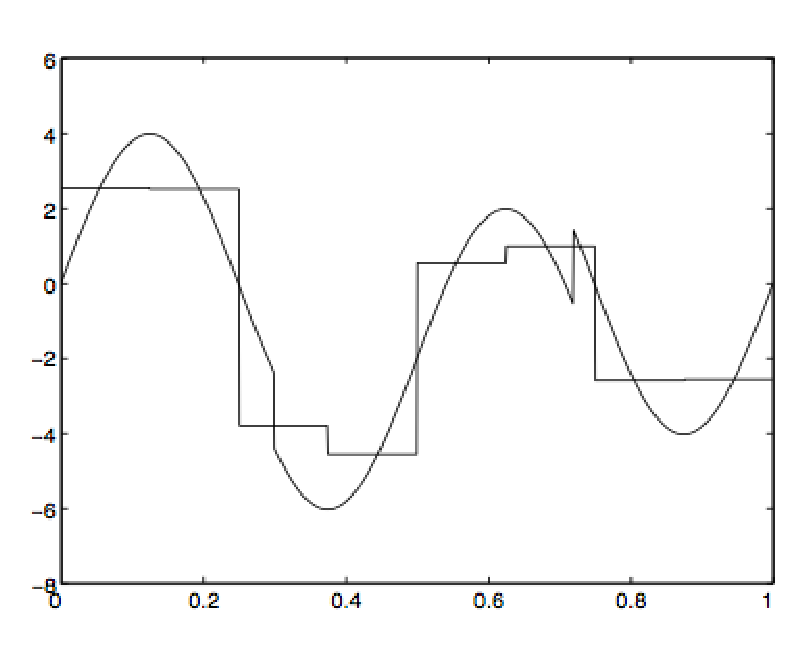
\includegraphics[width=100mm]{/Users/peter/honors/thesis/experiments/exp_features/figures/haarreconstruction.eps}
		\caption{Reconstruction from haar wavelet coefficients of a signal}
	\end{figure}
	
	The first 4 levels of granularity of Haar Wavelets will be used, giving 15 features in total (1 for the 1st level, 2 for the 2nd, 4 for the 3rd, and 8 for the 4th), as \verb#haar_n# for $n = 1 \ldots 15$. The transform requires that all datapoints are equally spaced in the time domain, the width of the signal is a power of 2, and there are no gaps. Both missing data and the short ends of the signal with be filled with 0s.
	

	
	\subsection{Lomb-Scargle periodogram}
	An implementation of the Lomb-Scargle periodogram based on the work in the paper \href{http://adsabs.harvard.edu/abs/1989ApJ...338..277P}{Fast algorithm for spectral analysis of unevenly sampled data} was taken from \url{http://www.astropython.org/blog/2010/9/Question-period-finding-packages-in-python}. This implementation allows us to extract as features the phase of significant peaks in the light curve and the intensity on these peaks. Computations are taken on centered (mean subtracted, divided by standard deviation) light curves and the top 5 frequences and their intensity are written as \verb#ls_phase(n)# and and \verb#ls_peak(n)# for $n = 1\ldots 5$. \\ % TODO add ref to paper
	
	\begin{figure}[ht!]
		\label{fig:lsspectrum}
		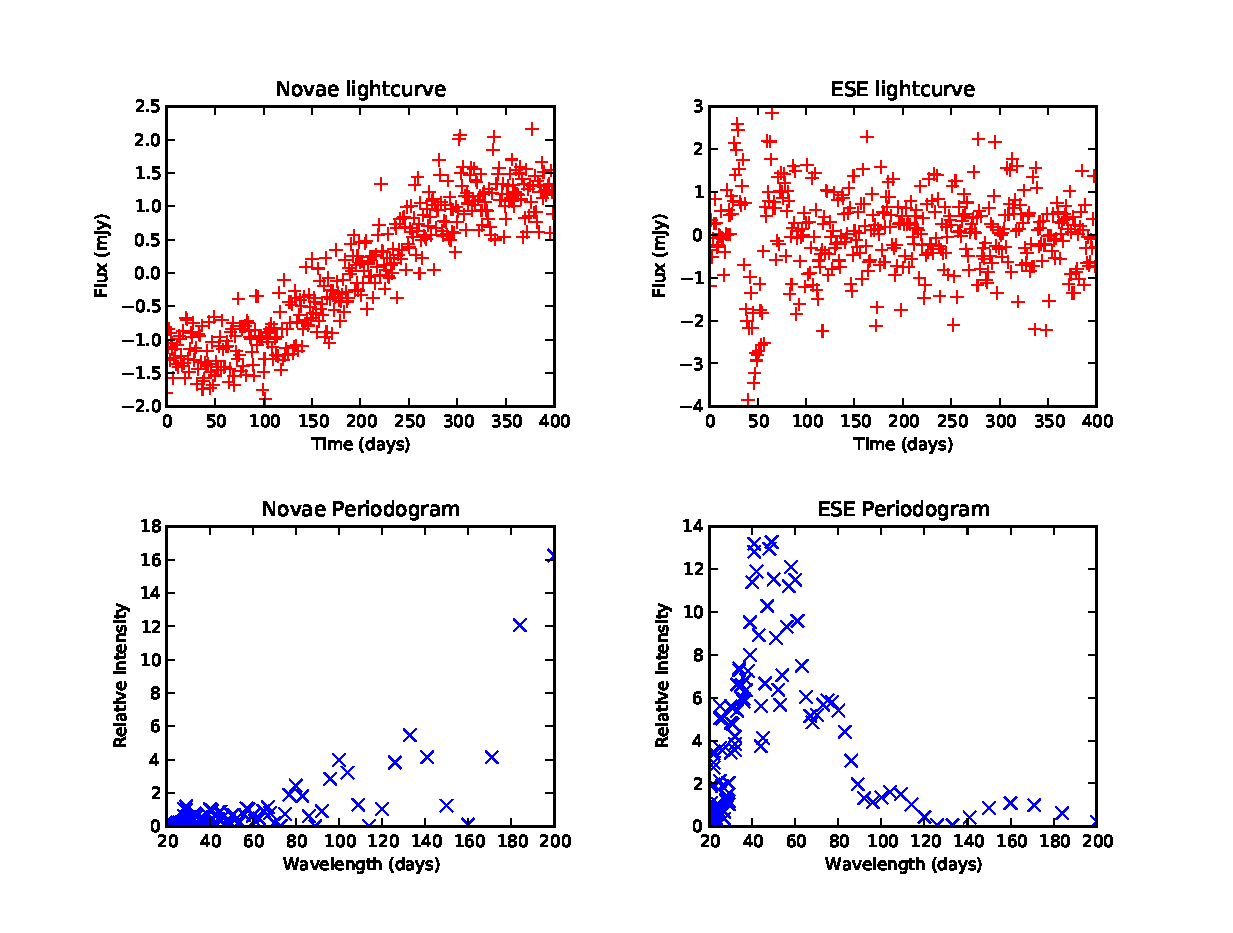
\includegraphics[width=120mm]{/Users/peter/honors/thesis/experiments/exp_features/figures/lomb_demo.eps}
		\caption{Spectrum produced by Lomb-Scargle periodogram for sample light curves}
	\end{figure}
	
	As they have little relation to the structure of the light curves, harmonics of wavelength less than 20 days and greater than 200 days are omitted.
	
	\section{Results}
	
	\section{Discussion}
%	\subsection{No distortions}
%	\subsection{Power law}
%	\subsection{Sparse data}
%	\subsection{On-line}
%	\subsection{All distortions}

	\section{Conclusion}
	
	% TODO 
	%\section{Other features}
	%\begin{itemize}
	%	\item ARMA coefficients
	%	\item Distance to profile light curves under various measures
	%	\item Some kind of segmentation profile distance
	%	\item Temporal grammar distance to profiles
	%	\item Shapelet profile distance
	%\end{itemize}
		
	%\section{Results} % TODO subtractive analysis 
	%\chapter{Results} \label{chap:results}

The results go here.


%	\section{Discussion}
%	\subsection{Baseline results}
%	The baseline results for this experiment come from the classification performance trained and tested on centered lightcurves with no distortions. An additional experiment to evaluate the impact of amplitude scaling involved training on centered light curves and testing on light curves with a power law distribution, as described in chapter two. \\ \\
%	The results demonstrate that basic statistical features are very good at discriminating amongst light curves with no noise and with a consistent distribution of signal intensity. The only points of confusion with the classifer are 10\% of both the supernova and X-ray binary light curves confused with each other, and another 10\% of the supernova light curves incorrectly classified as Novae. These confusions are not surprising since in a few cases these classes look a lot like each other. Additionally, the expected inherent extreme brightness of a source like a supernova is removed as a property when the data is centered. \\ \\ % TODO is this is a valid comment?
%	The experiment evaluating classification ability under the power law distribution gives similar results. There is a slightly pronounced confusion between the supernova, X-ray binary and nova classes, most likely due to the relative slopes of the important motifs of classes between increased (or lowered) under the amplitude scaling. In addition, there is a new mutual confusion between the background source and ESE classes of about 10\%, a a misclassification of the IDV class as Novae, SNe and XRB, and finally both SNe and XRB as Flare stars. From a flux distribution only point of view, and disregarding the time domain, ESEs and BGs do have very similar light curves. It is likely that before a power law distribution the variance and distribution around the median was what distinguished these 10\% of cases. A similar explanation applies to the other issues arising in this classification. Although not a catastrophic level of confusion, it is likely these results could be improved with the use of more sophisticated features in the time domain.  \\ \\ % TODO you need evidence to support these claims
%	
%	\begin{itemize}
%		\item Breakdown per each feature, explanation of why Haar wavelets do not resolve confusion. They should be excellent features for these data conditions.
%		\item Inclusion of light curve plots for cases which were confused
%		\item Specifics of f-score, recall and precision per class
%		\item Suggestions for improvement in terms of time domain features
%	\end{itemize}
%	
%	\subsection{Varying missing data}
%	\begin{itemize}
%		\item The classifier produces an ensemble of decision trees that effectively utilises the specific class discrimination strength of each
%		\item No particular feature is good at classifying all the classes, but usually is particularly good at one. Perhaps this should be examined in more detail to give some useful insight into the features.
%		\item Spectral features performed worst, which is strange given that they should be robust to missing data
%		\item The most basic features, the statistical metrics on the flux distribution, the slope properties and the haar coefficients, performed about the same. Median based features and flux percentiles performed second worst.
%		\item  The nature of the light curve plots at the extreme end of the distortion suggests that these results - a microaveraged F-Score of 0.4 for all the features - can be improved.
%		\item Again - why do Haar coefficients perform so poorly, when they should be quite powerful for this problem?
%		\item What are some suggestions for improvements on these features, in particular extensions to the time domain.
%		\item Confusion matrices indicate that all the data appears mostly like background noise, which is expected, but more unexpectedly a lot like ESEs, and to a lesser extent flare stars and XRB. Why is this the case?
%		\item Almost no novae or supernovae are classifier correctly at even moderate amounts of missing data (5 in 10 points removed). The plots show a very clear signal even at these distortion levels, so why the decrease?
%	\end{itemize}
%	
%	\subsection{Varying observed data}
%	
%	\subsection{Varying noise to signal variance ratio}
%	
%	\subsection{Varying observed data with a power law distribution, 1.5 noise to signal variance ratio and no missing data}
%	
%	\subsection{Varying observed data with a power law distribution and 1.5 noise to signal variance ratio and 1 in 10 data points missing}
%	
%	\subsection{Varying observed data with a power law distribution, 1.5 noise to signal variance ratio and 5 in 10 data points missing}
%	
%	\subsection{Varying observed data with a power law distribution, 1.5 noise to signal variance ratio and 9 in 10 data points missing}
%	
%	
%	\section{Future work}
%	
%	\section{Conclusion}
%\end{document}
